\subsection{Fuerza de Lorentz}

Una carga móvil con una velocidad \(\vec{v}\), en presencia tanto de un campo eléctrico \(\vec{E}\) como de un campo magnético \(\vec{B}\) es descrito por dos modelos de partícula en un campo. Experimenta a la vez una fuerza eléctrica \(\vec{F}_E=q\vec{E}\) y una fuerza magnética \(\vec{F}_B=q\vec{v} \times \vec{B}\). La fuerza total es la fuerza de Lorentz:

\begin{equation}
  \vec{F} = q\left(\vec{E} + \vec{v} \times \vec{B}\right)
  \label{eq:f_lorentz}
\end{equation}

\subsubsection{Fuerza magnética en un conductor}
\label{sec:fuerza_magnetica_en_un_conductor}

\begin{wrapfigure}{r}{0.3\textwidth}
  \centering
  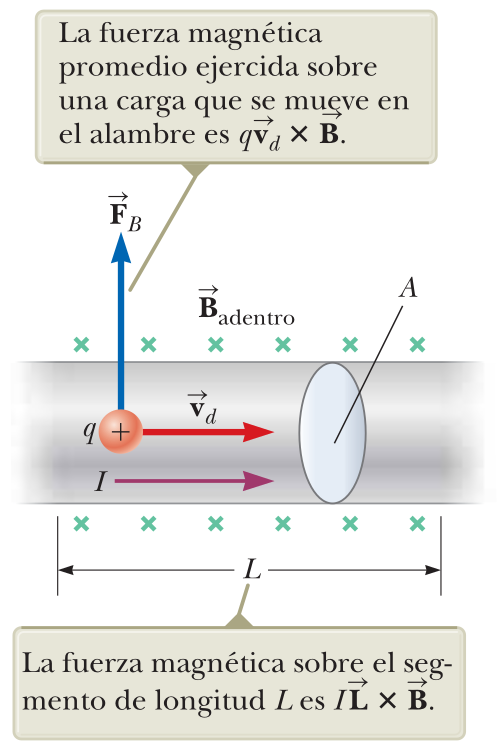
\includegraphics[width=0.3\textwidth]{lorentz.png}
  \caption{Un segmento de un alambre conduciendo corriente en un campo magnético \(\vec{B}\)}
  \label{fig:lorentz}
\end{wrapfigure}
Ahora hagamos un análisis de las fuerzas que interactúan para un cable conductor como el que se muestra en la figura \ref{fig:lorentz}. Vemos que en la figura el campo magnético es entrante. Si no circula corriente eléctrica, entonces no hay movimiento de cargas, por ende las cargas tendrán una \(v_d=0\) y la fuerza magnética será cero. Si hacemos circular cargas sobre el conductor aplicando una diferencia de potencial entre las puntas del conductor, entonces \(v_d \neq 0\) y por lo tanto existirá una fuerza magnética. 
Conviene cuantificar esta explicación considerando la longitud \(L\) del segmento y el área de sección transversal \(A\). Al tener en cuenta las dimensiones del cable, podemos expresar la \textbf{fuerza total} que sentirá el cable. Sabiendo que la corriente que circula por el cable es \(I = nq v_d A\) y el volumen del cable es \(AL\) entonces: 
\[
  \vec{F}_B = (q\vec{v}_d \times \vec{B})nAL
\]
Reemplazando \(I=qn \vec{v}_d A\) en la expresión:
\[
  \vec{F}_B = I\vec{L} \times \vec{B}
\]
donde \(\vec{L}\) es un vector que apunta en la dirección de la corriente \(I\) y tiene una magnitud igual a la longitud \(L\). Si se expresa el producto vectorial como el módulo de los vectores por el seno del ángulo entre ellos:
\begin{equation}
  \boxed{F_B = IL \cdot B \, \sin(\theta)}
  \label{eq:fuerza_magnetica_en_un_conductor}
\end{equation}